Suppose that $\boldsymbol{n}$ and $\boldsymbol{z}$ are transformed by $\boldsymbol{S}$. On the same axes as in the previous part, plot the vectors $\boldsymbol{Sn}$ and $\boldsymbol{Sz}$ using MATLAB.

\begin{solution} \
    \begin{lstlisting}[language=Matlab]
n = [-1; 1];
z = [-1; 1.01];
S = [2 1; 1 2];

Sn = S*n;
Sz = S*z;

hold on
quiver(0, 0, n(1), n(2));
quiver(0, 0, z(1), z(2));
quiver(0, 0, Sn(1), Sn(2));
quiver(0, 0, Sz(1), Sz(2));

legend('n', 'z', 'Sn', 'Sz')
    \end{lstlisting}
    \begin{center}
        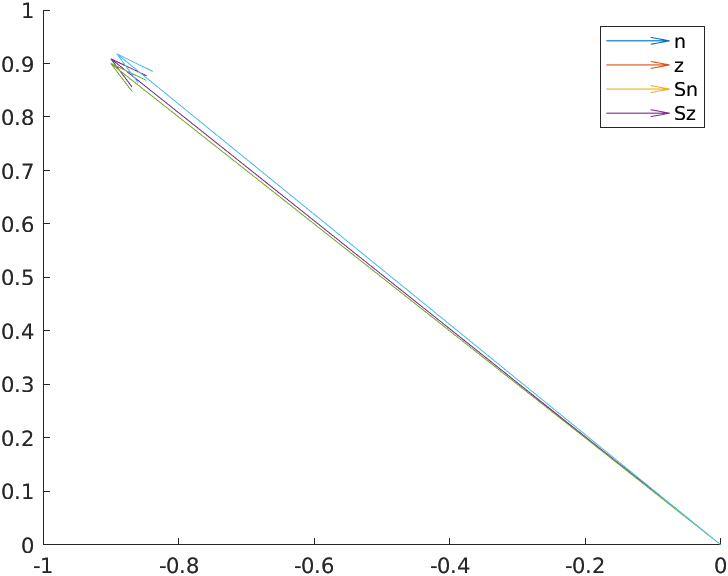
\includegraphics[width=0.7\textwidth]{img/e8p2.png}
    \end{center}
\end{solution}